The chip apparatus was assembled for preliminary tests, but isolated from the 
main \CaF{} experiment. This modest setup was useful for a variety of
measurements, which will be discussed below, including vacuum compatibility,
current testing under vacuum, and looking at the amount of background scatter
from the apparatus during imaging. We anticipate background scatter to be a
significant challenge in an experiment close to a surface, and discuss
possibilities for a background-free imaging scheme in
section~\ref{exper:bgf}.

\section{Experiment assembly}

In this section we will give details of the apparatus, especially the chip
flange assembly, which was introduced at the end of chapter~\ref{overview}. The
flange assembly is designed to hold the chip in position for loading \CaF{},
whilst also providing current delivery and heat sinking. Considerations have
been made for future experiments using microwaves, with two high-frequency
microwave feedthroughs incorporated as well. The flange was manufactured by
Allectra GmbH, and the heat sink was machined in the CCM workshop.  A detailed
view is shown in \myfigref{overview:fig:chipchamber}.

The copper heat sink is mounted to the flange using screws where the thread has
been partially removed. This is done to prevent any trapped gas causing virtual
leaks inside the chamber. The heat sink supports the subchip and also
incorporates the large U-trap, which is recessed beneath the chip. It is
electrically isolated from the heat sink by \AlN{} plates. This material is
chosen since it is an electrical insulator, but will still allow the conduction
of heat away from the U-wire whilst being UHV compatible. The subchip is
attached to the heat sink with metal screws. Since the conductor tracks come
very close to the mounting holes, we isolate the screws from the surface using
washers made from polyimide (another UHV compatible insulator) which were
manufactured in the CCM workshop.

The current is delivered to the U-wire through two high-current feedthroughs.
For the chip currents, the 16-pin feedthrough is used, and is connected to the
subchip by kapton-coated wires from LewVac. When connecting the wires to the
subchip we use polyimide bushings (also made in the CCM workshop) to ensure
that they are electrically isolated from the aluminium core of the PCB.

The flange is mounted in the chip chamber, which is a DN63 cube chamber from
Kurt J.  Lesker Co.\ (KJL) and whose configuration is shown in
\myfigref{exper:fig:exper}.  The assembly is designed so that molecules will
enter the chamber along an axis that is \SI{3}{\milli\meter} from the surface
of the chip. A tee is installed to allow for additional vacuum ports whilst
still allowing a clear line of sight across the chip surface. The direction of
the line of sight is shown in the figure by the pink arrow, and passes through
the anti-reflection coated viewports which also from KJL. This provides optical
access across the surface of the chip for illumination.  Onto the tee we attach
a Agilent TwissTorr 84 FS turbo pump, backed by a scroll (not pictured).  There
is also a DN63-DN40 adapter opposite the chip flange, this will be where the
chamber is attached to the \CaF{} experiment in the future, but for testing
purposes a pirani gauge or Leybold residual gas analyzer (RGA) is attached
instead.

\begin{figure}
  \centering
  \includegraphics[width=\textwidth]{figs/exper/exper.pdf}
  \caption{A top-down (a) and profile (b) view of the chip experiment. In (a)
  we show the line of sight through the chamber by the pink arrow. In (b) we
  show a view as if looking through the viewport on the tee, and also highlight
  the position of the interior lens inside the chamber. Here the
  pink arrow denotes the path of light collected for imaging from beneath the
  chip.}
  \label{exper:fig:exper}
\end{figure}

The optical access allows for two main styles of imaging experiment. In both, a
laser beam will enter through the viewports as shown in
\mysubfigref{exper:fig:exper}{a}. Light-induced fluorescence can then be imaged
by collecting the light along this axis. This would allow measurement of the
changing height of molecules that are released from the trap as they fall under
gravity. 
%
An alternative arrangement is shown in in \mysubfigref{exper:fig:exper}{b},
where light is collected from a viewport beneath the chip and imaged onto a
CCD. This may be useful since it avoids imaging along the path of the light
driving the transitions and could reduce background scatter. We anticipate
background scatter to be a significant problem for an experiment that is
conducted close to what essentially amounts to a giant mirror, and this scheme
will be discussed further in section~\ref{exper:scatter}.

Finally, we note that the current drivers for the experiment were not completed
as part of this project. Instead, a simple regulated power supply and
field-effect transistor (FET) switch were used to control current pulses for
testing. This will be discussed in section~\ref{exper:current}.

\section{Vacuum testing}

For testing the vacuum compatibility of the components, the RGA is attached to
the chamber. This is useful for diagnosing leaks and outgassing in the chamber.
To reach UHV pressures, it is required to bake the experiment.  Heater tape is
applied and the chamber is wrapped in foil, the temperature is then raised over
the course of a few hours to just over 100 degrees Celsius.  It is held at this
temperature for atleast 48 hours, before being ramped back down. This removes
excess water vapour from inside the chamber, and expels any water that has been
absorbed into the chamber walls. The exact parameters of the bake are recorded,
but it was found that following this approximate procedure was sufficient for
our purposes.

The chamber was first leak checked~\cite{PfeifferVacuum} and then brought to
UHV pressure with the chip flange assembly replaced with a blank. This provided
a baseline pressure for the chamber. We then swapped in the flange assembly,
and repeated the bakeout process with various iterations of our design. In our
design process we were careful to choose materials that are UHV compatible but
it was important to check that the assembly could reach the pressures required.
In particular we were concerned with the Epoxy Technology glue, since any
errors in the mixing and application procedure could cause outgassing, and the
solder, which was not rated for UHV uses.

To measure the pressure of the chamber an RGA scan is undertaken, with the
resulting partial pressures shown with and without the chip assembly in
\myfigref{exper:fig:rga}. The total pressure (the sum of the partial pressures)
is \SI{5.0E-10}{\milli\bar} and \SI{8.8E-10}{\milli\bar} in each case
respectively. The scan with the chip assembly has a similar shape to the empty
chamber scan, but with slightly higher values.  In both, we see the typical
peaks for hydrogen (2), water (18) and nitrogen (28), which dominate the
spectrum. This is typical of a scan through a UHV system~\cite{PfeifferVacuum},
and suggests that the chip assembly does not introduce any sources of
contamination or outgassing into the experiment.
%
Further tests were conducted when using a chip with wirebonds rather than
solder, and the microwave barrel connectors and launchers (see
section~\ref{mws:integrating}) which will be required for future experiments.
These yielded similar results to those discussed above, with no discernible
change in the pressure.

  \begin{figure}[htb]
  \centering
  \begin{tikzpicture}
    \begin{axis}[
        ymode=log,
        enlargelimits=true,
        xlabel=Mass number,
        ylabel=Partial pressure (\si{\milli\bar}),
        width=0.8\textwidth,
        height = 0.4\textwidth,
        legend pos=north east,
        x tick label style={/pgf/number format/.cd, set thousands separator={}},
        ylabel style={yshift=10pt}
    ]
      \addplot [thick, color=blue] table {figs/exper/rga/emptyData.dat};
      \addlegendentry{Empty chamber};
      \addplot [thick, color=pink] table {figs/exper/rga/chipData.dat};
      \addlegendentry{Chip assembly};
    \end{axis}
  \end{tikzpicture}
  \caption{RGA scan for the chip chamber assembly when empty, and when loaded
  with the chip flange assembly.}
  \label{exper:fig:rga}
\end{figure}


\section{Current testing}
\label{exper:current}

It was also important to test the currents that can be achieved through the
chip trapping wires. These tests were conducted with the chip under vacuum
($P<10^{-6}\si{\milli\bar}$) and using the setup shown in
\myfigref{exper:fig:curtest}, which was used since our custom current drivers
where not ready at this stage. A regulated power supply delivers a current to
the chip, controlled by the FET circuit that is in turn switched by a signal
generator. This gives us control over the pulse length, and allows us to
deliver voltage $V_\text{PSU}$ up to \SI{30}{\volt} to the chip, represnted
here by the resistor $R_\text{load}$. The current through the chip can be
measured via the potential difference across $R_\text{sense} = \SI{0.5}{\ohm}$.

\begin{figure}[htb]
  \centering
  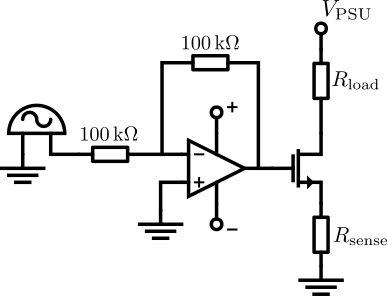
\includegraphics[width=0.5\textwidth]{figs/exper/circuit.pdf}
  \caption{The electronic circuit used to test the chip wires. The chip is
  represented by resistor $R_\text{load}$. The operational amplifier is powered
  by a separate power supply. This figure was produced using the assets from
  \inlineref{ElCompLib}.}
  \label{exper:fig:curtest}
\end{figure}

\subsection{Wirebond tests}

We originally tested a number of designs where the chip was connected to the
subchip with wirebonds using the method described in
section~\ref{fab:gluebond}. In these cases it was found that the wirebonds were
unreliable at high currents. It was possible to achieve pulses of several
amperes through even the small wires, but these were not reliably repeatable,
and often resulted in the wirebonds being broken.

These tests were conducted using a \SI{200}{\milli\second} pulse of current,
repeating every \SI{10}{\second}. The supply voltage was ramped up gradually,
and the current through the chip was measured via the potential difference
across the FET controller's sense resistor (see \myfigref{exper:fig:curtest}).
Several iterations of chips (with varying wire heights) were tested, using all
trapping wires. However no meaningful results for maximum attainable current
were found, as invariably the wirebonds would fail. This was eastablished by a
visual inspection of the chip, and checking the electrical continuity across
the trapping wires and from the subchip to the chip.

We attempted to improve the maximum current by increasing the number of
wirebonds on each pad, and by improving the quality of the wirebond joints. We
found that the former yielded an improvement to the maximum current capacity,
but the quality of the wirebond joints was difficult to quantify. As a rule of
thumb, the wirebonds were re-done if they could not withstand a light tug from
a pair of tweezers. Ultimately the number of wirebonds that it was possible to
produce was limited by the width of the wirebond pad, and the width of the
wirebonder head. We could achieve approximately ten wirebonds per pad somewhat
reliably.

There are various options that could be used to increase the maximum current of
the wirebonds.  We considered using a ribon wirebond, which promises
higher current throughput by using a ribon-shaped wire rather than a round one.
This was not possible due to the unavailabliity of the the hardware at LCN.
Another option was to use higher-diameter wire, but instead we attempted to
directly solder the chip, as described in the next section.

\subsection{Solder tests}

An alternative to wirebonding is to directly solder the chip to the subchip.
This must be done carefully, as described in section~\ref{fab:solder} but if
done correctly it yields a highly stable electrical connection. In the next
section I will demonstrate that this method is compatible with UHV. Current
tests were performed with the same apparatus as for the wirebonded chips, as
shown in \myfigref{exper:fig:curtest}. For solder joints, the results were
reliably repeatable, and we were able to observe sufficient current densities
for trapping (compared to those laid out in section~\ref{overview:design}).

We consider a typical example of testing using the small wire
(\SI{9}{\micro\meter}), on a chip where the wire height achieved was
\SI{9}{\micro\meter}. Again, the current was pulsed on for
\SI{200}{\milli\second} once every \SI{10}{\second}, which we imagine to be
representative of a typical experiment. We show the current through the chip as
a function of supply density in \mysubfigref{exper:fig:current}{a}. Also shown
is a linear fit to the first ten data points. We observe here that for low
voltages, the current obeys Ohm's law, as we would expect, but this diverges
for higher voltages, suggesting that heating occurs in the device.

% Data from 2022-04-06_thesis_currenttest.nb (and from there just OneNote)
\begin{figure}[htb]
  \centering
  \begin{subfigure}[b]{0.45\textwidth}
  \begin{tikzpicture}
    \begin{axis}[
        enlargelimits=true,
        xlabel=$V$ (volts),
        ylabel=$I$ (amperes),
        width=\textwidth,
        height = \textwidth,
        x tick label style={/pgf/number format/.cd, set thousands separator={}},
        ylabel style={yshift=-8pt}
    ]
        \addplot [thick, blue, only marks] coordinates { (0.5, 0.1)(1, 0.28)(1.5, 0.46)(2, 0.64)(3, 1.04)(3.5, 1.2)(4, 1.4)(5, 1.7)(6, 2.2)(7, 2.6)(8, 2.8)(9, 3.)(10, 3.4)(11, 3.6)(12, 4.)(13, 4.4)(14, 4.6)(15, 4.8)(16, 5.)(17, 5.4)(18, 5.6)(19, 6.)(20, 6.)(21, 6.4)(22, 6.6)(23, 6.6)(24, 6.8) };
        \addplot[thick, pink, mark=none] coordinates {(0,-0.1136) (24,9.025)};
        \node[] at (axis cs: 1,8.5) {(a)};
      \end{axis}
  \end{tikzpicture}
  \end{subfigure}
  %
  \begin{subfigure}[b]{0.45\textwidth}
  \begin{tikzpicture}
    \begin{axis}[
        enlargelimits=true,
        xlabel=$I$ (amperes),
        ylabel=$R$ (ohm),
        width=\textwidth,
        height = \textwidth,
        x tick label style={/pgf/number format/.cd, set thousands separator={}},
        ylabel style={yshift=-8pt}
    ]
        \addplot [thick, blue, only marks] coordinates {
            (0.1, 2.7138)(0.28, 2.71005)(0.46, 2.70983)(0.64,
  2.71315)(1.04, 2.7332)(1.2, 2.74611)(1.4, 2.76617)(1.7,
  2.80446)(2.2, 2.89012)(2.6, 2.97829)(2.8, 3.02893)(3.,
  3.08393)(3.4, 3.20705)(3.6, 3.27515)(4., 3.42447)(4.4,
  3.59126)(4.6, 3.6812)(4.8, 3.77551)(5., 3.87419)(5.4,
  4.08465)(5.6, 4.19643)(6., 4.43309)(6., 4.43309)(6.4,
  4.68722)(6.6, 4.82084)(6.6, 4.82084)(6.8, 4.95882)
};
        \node[] at (axis cs: 1,8.5) {(b)};
      \end{axis}
  \end{tikzpicture}
  \end{subfigure}
  \caption{Increasing current in the small chip wire. The current is shown as a
  function of supply voltage in (a). The pink line shows a linear fit to the
  first ten points. In (b) this is converted into a resistance (as described in
the main text), which increases for higher currents.}
  \label{exper:fig:current}
\end{figure}

Nonetheless, with sufficient voltage it is possible to achieve currents of
\SI{6.8}{\ampere}, which  corresponds to a current density of
$j=\SI{6.8}{\ampere}/(\SI{9}{\micro\meter}\times\SI{9}{\micro\meter})=
\SI{8.4E10}{\ampere\per\meter\squared}$. This is slightly higher than was
expected (see again section~\ref{overview:design}), and potentially not the
maximum current density achievable: we did not test this chip to the point of
failure as we wanted to preserve it and the required current for trapping had
already been met.

Further, the resistance of the chip as a function of current can be found by
fitting a third order polynomial to the $IV$ curve in
\mysubfigref{exper:fig:current}{a}, and taking its derivative. This derivative
approximates the chip's conductance at that voltage and current, the resistance
is easily found by taking the reciprocal of this conductance and the result is
shown in \mysubfigref{exper:fig:current}{b}. We see that for high $I$, the
resistance is increasing quadraticlly, and therefore assume that the wire is
nearing its point of failure.

\subsection{Wire failure}

During testing of another chip, we were able to pass sufficient current to
destroy the small wire, although this was during an early stage of the tests
and so the current at which this occurred was not properly recorded. However it
is useful to be able to distinguish a good wire from one that has been
destroyed by heating. These are shown in \myfigref{exper:fig:brokenwire}~(a)
and~(b) respectively.

\begin{figure}[htb]
  \centering
  %(a) good wire, (b) bad wire from OneNote 7 April
  \begin{subfigure}[b]{0.45\textwidth}
    \centering
    \begin{overpic}[width=\textwidth]{figs/exper/burn/good.png}
      \put(9,20){\SI{100}{\micro\meter}}
      \put(85, 70){(a)}
  \end{overpic}
  \end{subfigure}
  \hspace{1cm}
  \begin{subfigure}[b]{0.45\textwidth}
    \centering
  \begin{overpic}[width=\textwidth]{figs/exper/burn/bad.png}
      \put(9,20){\SI{100}{\micro\meter}}
    \put(85, 70){(b)}
  \end{overpic}
  \end{subfigure}
  \caption{A wire before (a) and after (b) destruction due to fusing under
    extreme current load. Note that the clearly defined edges and solid colour
    have changed to a wobbly and poorly-defined region. In bothsubfigures ,
    part of a fanout is also visible.
    }
  \label{exper:fig:brokenwire}
\end{figure}


\section{Scatter testing}
\label{exper:scatter}

In the existing \CaF{} experiment, the molecules can be imaged by light-induced
fluorescence.  The $X(v=0)\rightarrow A(v=0)$ transition is driven by
\pewpew{}{00}, and light is emitted as the molecules spontaneously decay from
$A$ back to $X$. Most molecules will decay back to $X(v=0)$, releasing a photon
at the same wavelength as the laser, which can be collected and imaged on a
CCD. Since the laser and fluorescence are at the same frequency, any light
scattered from the viewports or from nearby objects such as the quadrupole
coils will create a background that must be accounted for in post-processing.
Various steps are taken to reduce this background, which would otherwise
obscure any signal. Most notably the internals of the chamber are painted black
to reduce reflections. However it is not clear whether it will be possible to
blacken the chip without compromising its capacity to operate. We also
anticipate that scatter will be worse near the chip than in existing
experiments since it is highly reflective.

To investigate this, the imaging scheme shown in
\mysubfigref{exper:fig:exper}{b} was configured in the same way that will later
be used to image molecules.  A plano-convex lens with a focal length of
\SI{26}{\milli\meter} and diameter of \SI{2}{\inch} was installed inside the
chamber. This high numerical numerical aperture lens was chosen to collect as
much light from the molecules as possible. This is then imaged onto a Hamamatsu
ImagEM X2 EM-CCD camera C9100-23B using a second biconvex
\SI{100}{\milli\meter}-focal length lens, in a four-$f$ configuration. The
EM-CCD camera is chosen to be able to achieve large gain for small signals on
individual pixels. We use \SI{100}{\milli\second} exposure and $2\times2$
binning of the pixels.

Although we do not have access to molecules, we can still shine the laser
across the chip and observe the background scatter. We do this for various
positions of the beam with respect to the chip surface, controlling the height
with a micrometer screw gauge. Five images were taken at each beam position,
from which we subtracted a background image taken with the laser light off, and
then calculate the number of laser photons scattered onto the EM-CCD using the
equation
%
\begin{equation}
  \text{photon number} = \frac{N_\text{px} k}{G_\text{a}
    G_\text{EM}\eta}
\end{equation}
%
where $N_\text{px}$ is the pixel value, $k=2.2$ is the conversion factor in CCD
mode for our camera, $G_\text{a}=1$ is the analogue gain,
$G_\text{EM}=1$ is the EM gain and $\eta=0.95$ is the quantum efficiency of the
detector\footnote{The dark value offset of the camera is accounted for by the 
background subtraction.}.

The beam $1/e^2$ diameter is chosen to be \SI{500}{\micro\meter}, and we
normalise the number of photon scatters produced for a beam with power
\SI{10}{\milli\watt}, such as may typically be used in an experiment. The
results are shown in \myfigref{exper:fig:scatter}, note that we define the
positive direction to be below the chip's surface. The shape of the curve
indicates that the most scattering occurs when the laser strikes the heat sink,
but of most interest to us is that the scatter is significantly higher than we
would observe when imaging in, for example, the existing MOT chamber.

%%  Some notes from doing the analysis of my laser results
%along with the background when the laser is turned off (black line) and
%background scatter when using \pewpew{}{10} and \pewpew{}{01} in combination
%with a \SI{606}{\nano\meter} bandpass filter. This will be relevant to the
%background-free imaging scheme described in the next section. The chip is
%positioned at height $0$, and the positive direction is moving the beam away
%from the surface (towards the ground).

% This data is from 2021-11-30_bgfreeimg2.nb
% Now changed to scattertest_thesischeck.nb
% I removed the data from the other wavelengths because it's basically
% meaningless
\begin{figure}
  \centering
  \begin{tikzpicture}
    \begin{axis}[
        enlargelimits=true,
        xlabel=Position from chip (\si{\milli\meter}),
        ylabel=Normalised scatters ($\times 10^6$),
        width=0.8\textwidth,
        height = 0.4\textwidth,
        legend pos=north east,
        x tick label style={/pgf/number format/.cd, set thousands separator={}},
        ylabel style={yshift=10pt}
    ]
      \addplot [thick, color=black, only marks, error bars/y explicit, error bars/y dir=both] table [x=x, y=y, y error=err] {figs/exper/bgf2606.dat};
    \end{axis}
  \end{tikzpicture}
  \caption{Background scatter normalised for a \SI{10}{\milli\watt} beam for
  various distances from the chip surface. Positive is away from the chip,
negative is into the heatsink.}
  \label{exper:fig:scatter}
\end{figure}

In the existing experiment, we would expect that for a \SI{10}{\milli\watt}
beam and \SI{100}{\milli\second} exposure we would see only on the order of a
thousand scattered photons~\cite{Williams2018}. As such, we have moved far
beyond the limit in which we would normally image a MOT, where we typically
collect on the order of $10^6$ photons over a \SI{10}{\milli\second} exposure.
% From Hannah's thesis (pg 88), 10ms exposure, 3.4E4 photon/s/mol and ~10^4 mols
Instead we will image $\sim10$ molecules dropped from a magnetic trap, so can
expect significantly reduced fluorescence.  To reduce the number of background
photons, a background-free imaging scheme has been investigated, as is
discussed in the next section.

\section{Background-free imaging}
\label{exper:bgf}

One possible method of reducing background whilst imaging molecules is Raman
Resonance Optical Cycling (RROC), an background-free imaging scheme recently
proposed and demonstrated using \SrF{} in \inlineref{Shaw2021}. In this scheme,
off-diagonal ($v\neq v'$) vibrational transitions are driven to excite the
molecule, which will decay primarily on the diagonal ($v=v'$) transitions. The
off-diagonal transitions are separated from the diagonal ones by
$>\SI{10}{\tera\hertz}$, and so it is possible to use a bandpass filter to
exclude the imaging light from any measurement. For an ideal bandpass filter
this would remove any background from imaging light scattered by the apparatus.

This scheme is shown for \CaF{} in \myfigref{exper:fig:bgfreelevels}, where
the \pewpew{}{01} and \pewpew{}{10} light is used to drive the transitions at
\SI{585}{\nano\meter} and \SI{628}{\nano\meter} respectively (see
\mytableref{overview:table:lasers}). Fluorescence from the decay on the
\SI{606}{\nano\meter} transitions $v'=0\rightarrow v=0$ and $v'=1\rightarrow
v=1$ is isolated by a bandpass filter, and can be imaged without the usual
background scatter. The filter used here is a Semrock FF01-605/15-25, which
allows light of wavelength $605\pm{15}\si{\nano\meter}$ to pass through it.

\begin{figure}
  \centering
  \includegraphics[width=0.9\textwidth]{figs/energylevels/bgfree.pdf}
  \caption{
  The RROC scheme for \CaF{}. An optical cycle is established, with pumping on
  the $v=0 \rightarrow v'=1$ (gold) and $v=1 \rightarrow v'=0$ (red) transitions.
  Fluorescence from the $v=v'$ transitions (orange) is distinguished from the
  background by a bandpass filter before imaging.
  }
  \label{exper:fig:bgfreelevels}
\end{figure}

Reference~\cite{Shaw2021} reports a suppression of scattered light by a factor
of $\sim10^6$, and an average emission of 20 photons per molecule. In this
experiment, a beam of molecules was imaged, and this emission is limited by the
interaction time during travel. For imaging a stationary cloud of molecules we
would expect instead to be limited by the reduced scattering rate in the
off-diagonal transitions. In this section I will describe the technique, and
describe experiments conducted in a beam and in the MOT chamber.

\subsection{Calculating the scattering rate}

The scattering rates calculated in section~\ref{theory:cooltrap} can be modified to
apply to a multilevel system~\cite{Metcalf1999}. For a system with $n_e$
excited and $n_g$ ground states, which we assume are all connected with equal
strength (this can be ensured by applying a magnetic field to remix dark
states), there is a new effective linewidth~\cite{Williams2017}
%
\begin{equation}
  \Gamma_\text{eff} = \frac{2n_e}{n_g + n_e}\Gamma
\end{equation}
%
which arises because at saturation, the scattered particle spends approximately
the same amount of time in each of the states. Similarly there is an effective
intensity parameter,
%
\begin{equation}
  s_\text{eff} = \frac{2(n_g + n_e)}{n_g^2}.
\end{equation}
%

Making the substitutions $\Gamma\rightarrow\Gamma_\text{eff}$ and $s\rightarrow
s_\text{eff}$ into \myeqref{theory:eqn:scatteringrate} we have the scattering
rate between levels $v'$ and $v$ as
%
\begin{equation}
  R = \frac{s_\text{eff}\Gamma_\text{eff}}{1 + s_\text{eff} + \delta}.
\end{equation}
%
From now on we will take $\delta = 0$.

Notice that introducing $s_\text{eff}$ is equivalent to a change in the
saturation intensity
%
\begin{equation}
  I_\text{s, eff} = \frac{n_g^2}{2(n_g + n_e)}I_s.
\end{equation}
%
However we have made an implicit assumption that the transition being driven is
strongly coupled to the light, which is not true in the case of the
off-diagonal transitions. Here we are limited by the photon excitation rate,
which is
%
\begin{equation}
  R_\text{ex} = \frac{\Omega^2}{\Gamma}
\end{equation}
%
with $\Omega$ as the usual Rabi frequency, which we write in terms of the
dipole moment $\mathbf{d}$ and the electric field $\mathbf{E}$
%
\begin{equation}
  \hbar \Omega = \bra{g}\mathbf{d}\cdot\mathbf{E}\ket{g},
\end{equation}
%
where $\ket{g}$ and $\ket{e}$ are the ground and excited state of the
transition respectively.

The Rabi frequency can be estimated as follows, first take the orientation of
the molecule to be random with respect to the light field, so that the dot
product averages across the ensemble to give $dE/3$. Next, we consider the
matrix element $\bra{g}d\ket{e}$ as discussed in
section~\ref{theory:transitions}.  This term will contribute an electronic
factor ($d_e\SI{6}{\debye}$ for the $A\rightarrow X$ transition in \CaF{}), a
vibrational factor (the square root Franck-Condon factor $q_{v',v}$) and a
rotational part (approximately $1/\sqrt{3}$). The field amplitude is related to
the instnsity in the usual way, so the excitation rate is
%
\begin{equation}
  R_\text{ex} \approx \frac{2 d_e^2 q_{v',v}}{81 \hbar^2 c \epsilon_0 \Gamma}I.
\end{equation}

The relevant Franck-Condon factors are
%
\begin{align}
  q_{0,1} &= 0.03,\\
  q_{1,0} &= 0.015,\\
  q_{0,0} &\approx q_{1,1} \approx 1,
\end{align}
%
and since the off-diagonal transitions ($v' \neq v$) are a factor of $\sim100$
smaller than the diagonal transitions, an increase in the intensity of the same
factor is required to achieve the same scattering rates. Since the two
transitions are uncoupled, the total scattering rate for the RROC scheme will
be the lower of these two $R_\text{ex}$ values.

The \pewpew{}{01} laser used for the following experiments is the Spectra
Physics 380D, a single frequency ring dye laser, using Rhodamine 6G dye and
pumped by a Spectra Physics Millenia EV, a continuous wave diode-pumped solid
state laser. The power output from the 380D at \SI{585}{\nano\meter} is
expected to have a maximum of approximately \SI{300}{\milli\watt}, which means
that a \SI{1}{\milli\meter} diameter beam or smaller is required to saturate
the transition.  Due to this limitation we performed two experiments:
identifying the transition in the \CaF{} beam using a narrow laser beam waist,
and imaging the \CaF{} cloud in the MOT chamber with a \SI{5}{\milli\meter}
$1/e^2$ diameter waist.

\subsection{Identifying the transition frequency}

In this first experiment \pewpew{}{01} was used to identify the $X(v=0)
\rightarrow A(v=1)$ transition frequency. A pulsed beam of \CaF{} was addressed
with \pewpew{}{01}, with the laser frequency scanned between pulses.  When the
laser is at resonance it drives the transition and light-induced fluorescence
can be observed. The apparatus is shown in \myfigref{exper:fig:beamapp}, with
subfigure (a) showing the layout of the \pewpew{}{01} laser system. The
majority of the light passes through an electo-optic moldulator, which is used
to add the sidebands for addressing the hyperfine structure of the $X(v=0)$
state, and an acousto-optic modulator (AOM) which is used for switching. In
this experiment the EOM is switched off, and the AOM is not installed as
switching is not required.

\begin{figure}
  \centering
  \includegraphics[width=\textwidth]{figs/exper/beamexper_reduced.pdf}
  \caption{The optical (a) and vacuum (b) setup for the spectroscopy
    experiments. The dye jet (orange) is pumped (green
    arrow) to produce \pewpew{}{01} (yellow arrow). Beamsplitters (BS) are used
    to generate pick offs from the main beam. These are used for locking to the
    reference cavities, analysis with the wavemeter and comparision to IR light
    (pink arrow). The latter of these is achieved using the dichroic mirrors
    (DM) and  the scanning cavity as described in the main text. In (b) the
    buffer-gas source and \CaF{} beam are shown
    (c.f.~\myfigref{overview:fig:CaFcartoon}). The \pewpew{}{01} light is
    incident on the beam to inudce fluorescence, which is detected with a PMT,
    mounted above the beam (out of the page).
  }
  \label{exper:fig:beamapp} 
\end{figure}

The laser frequency is locked by the Spectra stable lock cavities. These
consist of one reference cavity and one scanning cavity. The light passes
through these and is measured on a photodiode. This signal is fed back to the
laser to control the cavity length and the laser frequency. This provides
stabilisation down to the \SI{100}{\mega\hertz} level. For more precise locking
of the laser frequency, we reference \pewpew{}{01} to the $F=2 \rightarrow
F'=2, 3$ cross-over feature of the \esRb{} $D_2$ line via a separate reference
laser. The frequency offset lock used to achieve this is described in
\inlineref{Jurgilas2021}. This infrared (IR) reference light is combined with
the \pewpew{}{01} beam using  a dichroic mirror (DM). This beam is then passed
through a scanning cavity, before being split into the two frequency components
on a second DM. We then observe the relative location of the transmission peaks
across the cavity scan, and can use a feedback loop to lock the dye laser to
the reference by transfer cavity lock (also described in
\inlineref{Jurgilas2021}). Further referencing is possible by a pickoff to a
wavemeter. % TODO Name of wavemeter?

A buffer-gas source  was used to produce the pulsed \CaF{} beam.  This
experiment was undertaken on a separate \CaF{} source to the one used on the
main beamline that was descibed in section~\ref{overview:existing}, but it is
functionally identical.  The beam was driven by \pewpew{}{01} with beam
diameter \SI{500}{\micro\meter} and power \SI{100}{\milli\watt}.  Light-induced
fluorescence was collected by a lens onto a photo-multiplier tube (PMT) mounted
above the beamline, as shown in \mysubfigref{exper:fig:beamapp}{b}.

The laser frequency was scanned from \SI{512.0725}{\tera\hertz} to
\SI{512.0750}{\tera\hertz} in \SI{25}{\mega\hertz} intervals. At each
frequency the total signal on the PMT is measured, using the Semrock
bandpass filter to remove background signal. This is shown in
figure~\ref{exerp:fig:beamresult}, where we can see that there are two clear
peaks. We interpret the large peak to be due to resonance with the $F=0$, $1^+$
and $2$ hyperfine levels, which we cannot resolve individually. We attribute
the second peak to the $F=1^-$ hyperfine level. This confirms that we are
capable of 

% From Mathematica 20201019_maybewrongfile.nb
% Incidentally, it was the right file...
\begin{figure}[htb]
  \centering
  \begin{tikzpicture}
    \begin{axis}[
        enlargelimits=true,
        xlabel=Laser frequency (\si{\tera\hertz},
        ylabel=PMT signal (\si{\volt}),
        width=0.8\textwidth,
        height = 0.4\textwidth,
        x tick label style={/pgf/number format/.cd, set thousands separator={}}
        %ylabel style={yshift=10pt}
    ]
      \addplot [thick, color=black] table {figs/exper/findtransition.dat};
    \end{axis}
  \end{tikzpicture}
  \caption{}
  \label{exper:fig:beamresult}
\end{figure}

\subsubsection{Attempt to image the \CaF{} cloud}

Having identified the $X(v=0)\rightarrow A(=1)$ transition frequency, we
attempted to use the RROC scheme to image a cloud of \CaF{} molecules in the
MOT chamber described in section~\ref{overview:existing}. In this experiment
the main \CaF{} buffer-gas source was used. The molecules underwebt the usual
slowing procedures described above, to create a \SI{50}{\micro\kelvin} cloud
with diameter of approximately \SI{3}{\milli\meter}. The cloud is then imaged
by using a combination of the \pewpew{}{01} and \pewpew{10} light.

The former is controlled using the same system as described above, but with the
EOM now turned on and overdriven, so as to produce the required sidebands to
address each hyeprfine state of $X(v=0)$ (see chapter~\ref{overview} and for
example \inlineref{Truppe2017}). In addition the AOM is installed and used to
switch the beam on and off. When powered, the majority of the beam is
defclected into the first order mode of the AOM, which is coupled into a fibre
and brought to the experiment for imaging. Otherwise the beam passes straight
through the centre of the AOM and is blocked. At the chamber, the beam is
expanded to \SI{5}{\milli\meter} diameter and passes through the centre of the
chamber before being retro-reflected to increase the power delivery and avoid
pusing molecules with the beam. 
%
The \pewpew{10} light is provided by the molasses beams.

In this experiment we create a MOT, and then switch off the magnetic field to
create a molasses. We hold the molecules in the molasses for
\SI{20}{\milli\second}, during which time an image of the flourescence is taken
using a Hamamatsu Orca R2 CCD camera.
% NOTE Sarunas wrote about the imaging system in his thesis that I can ref
The exposure last \SI{10}{\milli\second}. Following which \pewpew{}{00} is
switched off, and \pewpew{}{01} is switched on, along with a \SI{1}{\gauss}
magnetic bias field.  The direction of the field is chosen to ensure that the
molecules are not pumped into a state that is dark to \pewpew{}{01}, which
could otherwise occur due to the light's polarisation. A second
\SI{10}{\milli\second} exposure is then taken with the camera to image the
flourescence in the RROC scheme.

Due to expanding the beam to a much larger diameter (\SI{5}{\milli\meter} as
opposed to the \SI{500}{\micro\meter}), the intensity of the light is a factor
of 100 lower than in the previous experiment. Despite scanning the frequency of
\pewpew{}{01} across the same range as before, it was not possible to drive the
transition sufficiently for imaging. This result was somewhat anticipated, as
was reported in \inlineref{Shaw2021}, much higher laser power is required for
the RROC scheme than in conventional flourescence imaging. However it was
not clear before starting whether the background would be sufficiently low to
observe the transition in this experiment.

\section{Summary}

To summaries the results of this chapter, I have shown that the molecule chip
experiment is compatible with ultra-high vacuum conditions required for the
\CaF{} experiment, and that sufficient current can be achieved to create the
traps that were described and simulated in chapter~\ref{sim}. The chip trap is
therefore ready for loading with \CaF{} molecules. These molecules could be
imaged with an optical cycling scheme to reduce background scatter. I have
tested such a scheme in a \CaF{} beam where it was possible to resolve the
required $X(v=0)\rightarrow A(v=1)$ transition, but due to the limited power of
the laser used it was not possible to successfully implement the scheme for a
cloud of cold molecules.
